
% SIMT
This section covers the execution model of the GPU.
Based on Michael J. Flynn proposed Flynn's taxonomy \cite{Flynn1972}, used to identify computer architectures execution models, four categories were defined:

\begin{itemize}
	\item \textit{Single Instruction, Single Data} (SISD)
	\item \textit{Single Instruction, Multiple Data} (SIMD)
	\item \textit{Multiple Instruction, Single Data} (MISD)
	\item \textit{Multiple Instruction, Multiple Data} (MIMD)
\end{itemize}

The idea is to define how many instructions is performed on how much data.
For instance, SISD only allows for one instruction to be peformed on a single data input at a time, corresponding to a single-core CPU.
Based on SIMD, Nvidia introduced a new execution model \cite{Nvidia2009}, known as \textit{Single Instruction, Multiple Threads} (SIMT).
Now, lets see how this concept is mapped to the GPU architecture:


% Blocks -> Global Scheduler
A function running on the GPU is defined as a \textit{Kernel} (further descirbed in \cref{sec-pm-kernels}).
Once a Kernel is executed on the GPU, it is potentially handled by thousands of lightweighted threads running simultaneously.
As described in \cref{sec-hw-gpu-arhchitecture}, threads are grouped into \textit{thread blocks}, which are to be executed on SMs.
Once threads are divided into blocks, the blocks are dispatched by the Global Scheduler onto the SMs for execution.
A single SM can be assigned with multiple blocks, depending on the SMs limitations such as its memory.
In the case of multiple blocks assigned to a SM, the memory resources of the SM is divided evenly among the blocks.
\\\\
\textbf{Thread Assignment (Warps) -} Within the SM, the SIMT execution model is handled out by further organize the threads within the thread blocks into execution groups which is referenced to as SIMT units.
These SIMT units are better known as \textbf{Warps} using Nvidia terminology \cite{Nvidia2009} or Wavefronts by AMD \cite{Johansson2010}.
As the therm Warps is the mostly used, it is chosen for SIMT units throughout this report.
By the definition of the SIMT execution model, all threads within a warp is executed together, sharing the same instruction.
The main reason for grouping threads into warps, is to limit the amount of memory transactions performed by threads.
When threads have to access the Global Memory, the Warps are responsible for performing reads or writes for each thread within the warp, and in that way reduce the number of transactions performed.
The size of a warp is fixed to 32 threads/warp for all Nvidia GPU architectures \cite{Li2016}.
\\\\
\textbf{Thread Scheduling -} Scheduling of the warps is done by the Warp  Scheduler located within each SM.
As a warp is created, it is assigned to a warp scheduler, which it is assigned to for its remaining lifetime.
Each Warp Scheduler contains one or more Instruction Dispatch Units, which can be used to dispatch multiple different instructions at a time.
Depending on the architecture, the number of Warp Schedulers and Instruction Dispatch Units within a SM varies, however a conceptual example is used to illustrate how warp scheduling works.

\Cref{fig:hw-warp-scheduling} shows a scenario with a single Warp Scheduler, containing two Instruction Dispatch Units. 
In the example presented on the figure, the Warp Scheduler selects a warp, for instance the yellow marked Warp number 4 and splits it into two "half warps".
It hereafter executes two different Instruction to the two halfs, which are dispatched to execution on the SPs and/or SFUs.
However, this requires that the instructions handed out by the warps is executable by only half a warp.
Next, a new available warp is scheduled with a new set of instructions.
This rotation is continued until all instructions are executed.

\begin{figure}[ht]
	\centering
	\fbox{
		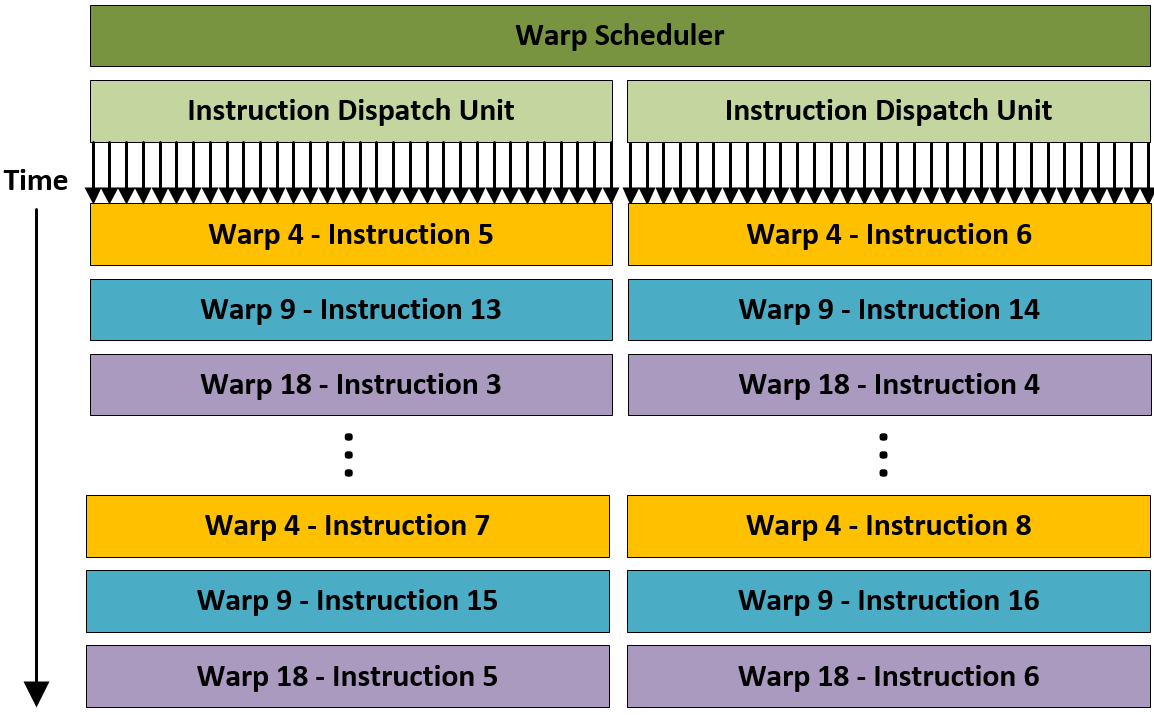
\includegraphics[width=0.8\textwidth]{figs/hw/hw-warp-scheduling}}
	\caption{Warp Scheduling}
	\label{fig:hw-warp-scheduling}
\end{figure}

Again, some architectures only contains one Instruction Dispatch Unit per Warp Scheduler, limiting the number of instructions that a warp can perform to one for all threads.

Prior to execution, instructions are located in a instruction queue, accessible to the Warp scheduler.
The warp scheduler is responsible of selecting the instructions that should be executed during the next clock cycle.
This selection is done based on two parameters, the status and priority of the instruction.

The status of an instruction is determined by its status flag, which can either be "ready" or "not ready".
When loaded into the instruction queue, an instructions flag is set to "not ready".
Once all operand and memory areas needed by the instruction is available, its status is changed to "ready".
The priority of an instruction is determined using a round-robin algorithm, which bases its decision on several different factors.

The instruction with the highest priority, and status flag set to "ready" is selected for execution by the Warp Scheduler.
\\\\
\textbf{Warp Divergence -} The SIMT execution model, however comes with a drawback.
In order to execute code where threads within the same warp is wished to perform different operations their SP cores have to diverge.
By diverge, it is meant that some cores are running instructions which they have in common, while others not having the same instructions remain idle and so on.
Such a code example could be a \textit{if-else} sentence as illustrated on
\autoref{lst:threaddiv} \& \cref{fig:hw-warp-div}.

\begin{lstlisting}[language=C,caption={Devergence generating code},label=lst:threaddiv]
if (threadId/2 == 0) {"Then"} 
else {"Else"}
\end{lstlisting}

 
\begin{figure}[ht]
	\centering
	\fbox{
		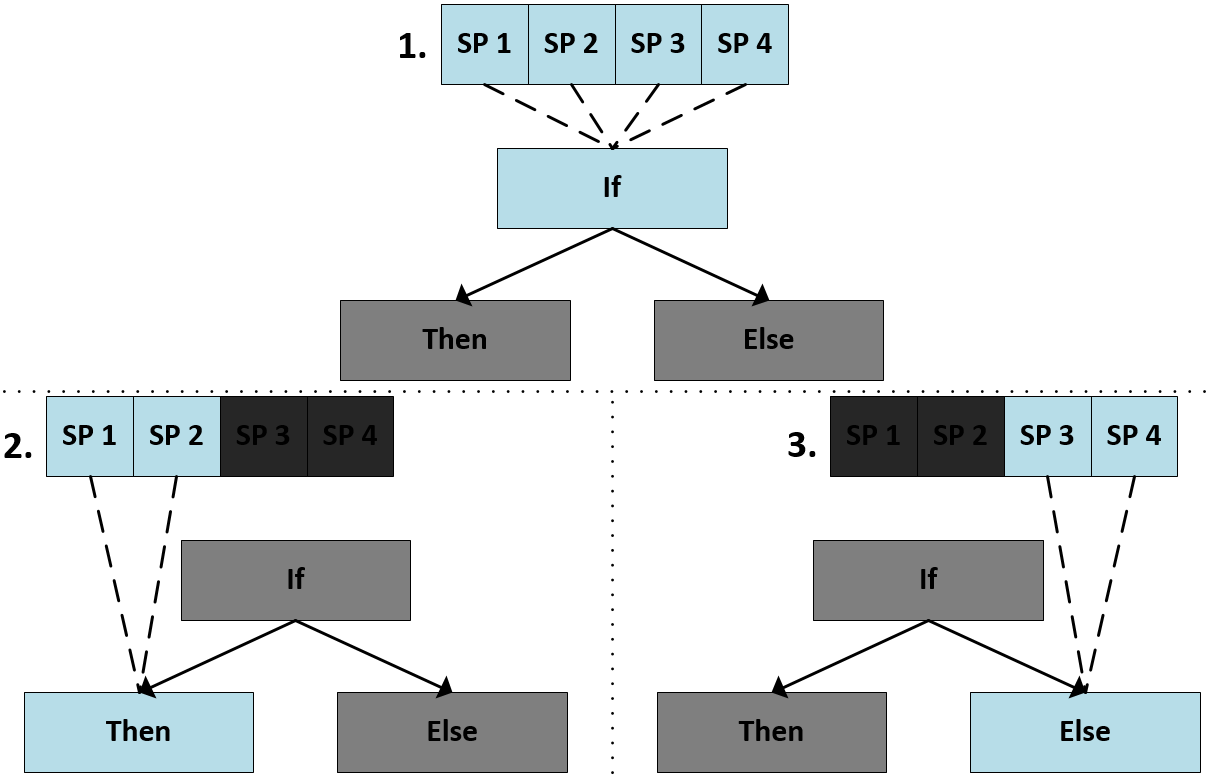
\includegraphics[width=0.7\textwidth]{figs/hw/hw-warp-div}}
	\caption{Warp Divergence}
	\label{fig:hw-warp-div}
\end{figure}

Here, first all threads test the \textit{if} condition.
Hereafter, threads running on SP1 \& SP2 executes the \textit{then} operation, while the other SPs remain idle.
Lastly, SP3 \& SP4 executes the \textit{else}, while SP1 \& SP2 idles.

This concept, defined as \textbf{Warp Divergence} obviously leads to performance losses, however \cref{ch-opti-intro} presents optimization aspects to this issue. 






